\documentclass{article}
\usepackage{tikz}
\usepackage[american]{circuitikz}

\usetikzlibrary{arrows,decorations.markings}

\title{Computer Organization and Architecture}
\author{Conrad A. Mearns}

\begin{document}

\maketitle

\noindent
\Large Turing Machines
\normalsize
\begin{enumerate}
  \item {Turing's Thesis: Every computation can be represented with a Turing Machine.}
  \item {Turing Machine: A mathematical model of a device that can preform any computation.}
  \item {Universal Turing Machine: A machine to implement any and all Turing Machines.}
\end{enumerate}

Beyond models, real world constraints include time, financial cost, power, security, thermal dissapation, space, etc.\\

\noindent
\Large Bits, Data Types, and Operators\\
\normalsize
\indent
The electro-magnetic field is not digital, yet all of modern computing is represented digitally. To compromise, 0 is a representation of the absence of voltage and 1 is a representation of the presence of voltage.

\centering
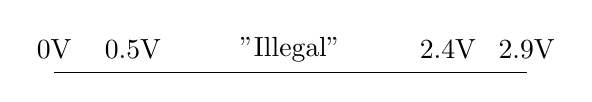
\begin{tikzpicture}
  \node (a) at (0,1) {0V};
  \node (b) at (1,1) {0.5V};
  \node (c) at (5,1) {2.4V};
  \node (d) at (6,1) {2.9V};
  \node (b) at (3,1) {"Illegal"};
  \draw (0,.7) -- (6,.7);
\end{tikzpicture}
\raggedright

\noindent
\Large
Signed Binary Arithmetic\\
\normalsize
\indent
Binary, without the addition of extra mathematical symbols, can only represent positive whole integers. Signed numbers like $-5$ require a formal system of representation in order to be used. A binary number can represent $2^n$ values for $n$ bits. The objective of signed numbers is to partition half of those values for negative number representation ($-2^{n-1}-1 \to -1$) and the other half to positive numbers ($1 \to 2^{n-1}$) while leaving zero and potentially one other number available.

\begin{enumerate}
  \item {
  Sign-Magnitude\\
  The most significant bit is 0 for positive values and 1 for negative values.\\
  $00101 = 5$ and $10101 = -5$
  }
  \item {
  One's Complement\\
  All bits are inversed to represent negative numbers. Like Sign-Magnitude, the most significant bit will tell you whether a number is positive or negative.\\
  $00101 = 5$ and $11010 = -5$
  }
  \item {
  Two's Complement (currently in use)\\
  For each positive number $A$, it's negative number ($B$) satisfies the equation $A + B = 0$ when the final carried bit is dropped. To get this number, take the One's Complement of $A$ and add 1.
  $00101 = 5$ and the One's Complement is $11010$. So the Two's Complement is $11011$. As proof, $00101 + 11011 = 100000$ but the last carried one is dropped, leaving $00000$.
  }
\end{enumerate}

\noindent
\Large
Arithmetic and Logical Operations\\
\normalsize
\noindent
Arithmetic operations
\begin{enumerate}
  \item {Addition\\Just addition, regardless if signed or not. Ignore the final carry-out.}
  \item {Subtraction\\First negate the second operand ($5 \to -5 for example$), then use addition.}
  \item {Sign Extension\\To add numbers, they must have the same number of bits. This is because of signed numbers, and storage.}
\end{enumerate}

\noindent
Overflow occurs when
\begin{enumerate}
  \item Signs of the operands are the same
  \item The sign of the sum is different
\end{enumerate}
\noindent
The issue can be tested for by examining the most significant bit's sign between the operands and the result.

\noindent
Logical operations
\begin{enumerate}
  \item {AND\\The result is true if and only if both operands are true.\\Useful for clearing bits, a mask of 1's signify keep.}
  \item {OR\\The result is true if either operand is true.\\Useful for setting bits. 1's in the second operand copy to the result.}
  \item {NOT\\The result is true if and only if the operand is false.}
\end{enumerate}
\noindent
Each operation is executed on each bit individually.

\noindent
\Large
Fractions, Floating, and Fixed-Point Values\\
\normalsize
\indent
A "binary" point is abstractly added to the value. To the left of the point, each bit is worth is $2^{-n}$ where n is the place left of the point. For example, $101.11$.

For large numbers, we use scientific notation. $Sign * (Fraction * 2^{Exponent})$
IEEE 754 Floating Point Standard for 32-bits signifies 1 bit for sign, 8 bits for the exponenant, and 23 bits for the fraction.
$1-01111110-10000000000000000000000 = -1.5*2^{???}$

\noindent
\Large
Other Date Types
\normalsize
\indent
\begin{enumerate}
  \item Single characters use ASCII to map 128 characters to 7-bit code.
  \item Text strings are sequences of characters often with a NULL to terminate. No hardware support.
  \item Images are arrays of images. Often has hardware support.
  \item Sound is a sequence of fixed-point numbers.
  \item Other data types my be defined abstractly by us and interpreted as needed.
\end{enumerate}

\noindent
\Large
Transistors\\
\normalsize
\indent
Each transistor is a digital switch. When combined in different circuits, transitor combinations can emulate certain logical operations such as AND, OR, and NOT. These can then be combined to create adders, multiplexers, decoders, and other farther complex structures.\\
Gordon Moore, an early founder of Intel, hypothesized that transistor count would double every two years. This is now known as Moore's Law.\\
Transitors have 3 wells. A well is a homogeneous material that is either more or less positive than negative. A negative well is denoted $n$ and a positive well is denoted $p$. The gate in a transitor creates a field to allow or dissallow charge to migrate across wells.

\noindent
n-Type Transistor (npn)\\
Two $n$ wells inside a large $p$ substrate.
\begin{itemize}
  \item When gate is tied to GND, the switch is open.\\
    No current flows from the source to the drain.\\
    '0 state'
  \item When gate is tied to voltage the switch is closed.\\
    Current flows from the source to the drain.\\
    '1 state'
\end{itemize}

\noindent
p-Type Transistor (pnp)\\
Two $p$ wells inside a large $n$ substrate.
\begin{itemize}
  \item When gate is tied to GND, the switch is closed.\\
    Current flows from the source to the drain.\\
    '1 state'
  \item When gate is tied to voltage the switch is open.\\
    No current flows from the source to the drain.\\
    '0 state'
\end{itemize}

\noindent
\Large
Complementary Metal Oxide Semiconductor Circuits(CMOS)\\
\normalsize
\begin{itemize}
  \item NOT Gate (Inverter)
  \item NOR Gate (NOT OR, Serial on top, Parallel on bottom)
  \item OR Gate (NOR + NOT)
  \item NAND Gate (NOT AND, Parallel on top, Series on bottom)
  \item AND Gate (NAND + NOT)
\end{itemize}

\noindent
\Large
Simplified Gates\\
\normalsize

\begin{itemize}
  \item {
  NOT Gate\\
  \begin{circuitikz}
    \draw (0,0) node[not port]{} (2,0);
  \end{circuitikz}
  }
  \item {
  OR Gate\\
  \begin{circuitikz}
    \draw (0,0) node[or port]{} (2,0);
  \end{circuitikz}
  }
  \item {
  NOR Gate\\
  \begin{circuitikz}
    \draw (0,0) node[nor port]{} (2,0);
  \end{circuitikz}
  }
  \item {
  AND Gate\\
  \begin{circuitikz}
    \draw (0,0) node[and port]{} (2,0);
  \end{circuitikz}
  }
  \item {
  NAND Gate\\
  \begin{circuitikz}
    \draw (0,0) node[nand port]{} (2,0);
  \end{circuitikz}
  }
\end{itemize}

\noindent
\Large
Other Circuits\\
\normalsize
\begin{itemize}
  \item 2-Bit Decoder\\
    Uses 4 AND Gates with different inverter configurations on each. It maps 2 inputs to 4 outputs.
  \item Multiplexer\\
  Uses 4 inputs and interprets to 1 output. A selector input of two wires will change the output from 4 AND Gates.
  \item Full Adder\\
    Capable of adding two bits with carry-in. Produces a one-bit sum with carry-out
\end{itemize}

\noindent
\Large
Logical Completeness\\
\normalsize
\indent
Can complete any truth table with just AND, OR, NOT. First, mark every output row that has a truth value of true. Draw an OR gate at the bottom to accept all true outputs. Connect AND Gates to the OR Gate and have every input connect to each AND gate. For each AND Gate, configure the inputs with invertes so that each AND Gate emulates a truth table row.

\noindent
\Large
Combinational vs Sequential Circuits\\
\normalsize
\noindent
Combinational Circuit\\
always produces the same output for a given set of inputs\\
Sequential Circuit\\
Stores information\\
Output depends on stored information (state) plus input

\noindent
\Large
R-S Latch\\
\normalsize
\noindent
R is used to 'Reset' or clear the element - set it to zero.\\
S is used to 'set' the element - set it to one.\\
If both R and S are one, the output could be either one or zero. To assert one of the inputs, use Active Low Logic.\\

\noindent
\Large
Gated D Latch\\
\normalsize
\noindent
Based upon R-S Latch and has 2 inputs. D (for data) and WE (write enabled). Two AND gates feed into the R and S inputs of an R-S latch, and input is only sent to the R-S latch when WE is asserted.\\
WE = 1 $\to$ latch is set to the value of D. S = NOT(D), R = D\\
WE = 0 $\to$ latch holds previous value. S = R = 1\\

\noindent
\Large
Register\\
\normalsize
\noindent
Side by side Gated D latches that share a single WE line, but has seperate data lines.\\
A register holds a n-bit value, controlled by a common WE.\\

\noindent
\Large
Memory\\
\normalsize
\noindent
Address is taken as multple inputs, that input passes to an address decoder which uses AND gates to specify what memory location can be written to, when WE is asserted.\\
Not the most expensive, and more transistors are needed in greater desnity.\\
Address decoder\\
Word Select Line\\
Word Write Enable

\noindent
\Large
Representing Multi-bit Numbers\\
\normalsize
\noindent
Number bits from right to left for convention. Use brackets to denote range.\\
D[l:r] denotes bit l to bit r from left to right in register D\\
May also see "A<14:9>"\\

\noindent
\Large
State Machine\\
\normalsize
\noindent
Finite State Machine with Datapath (FSMD)\\
Controller / Data Path\\
Another type of combinational logic with storage. It "Remembers" states and changes it's output(s) are based on inputs and the state machine's current state. This type of circuit is the heart of the controller in a CPU.\\

Combinational vs Sequential: Combinational types depend only on the values. Sequential types sctrictly depend on the order of values inputted.

The state of a system is a snapshot of all the relevant elements of the system at the moment the snapshot is taken.

State diagrams are directed graphs that show how actions change states.

\begin{enumerate}
  \item A finite number of states
  \item A finite number of external inputs
  \item A finite number of external outputs
  \item An explicit specification of all state transitions
  \item An explicit specification of what determines each external value
\end{enumerate}

Clock cycles are used in digital circuits to trigger state transitions. A single cycle is when the value changes between '1' and '0' fully. Transitions can be triggered with edge triggered logic, or level triggered logic.

Storage for state machines can be accomplished using a Master-Slave flipflop.

\end{document}
